\documentclass{article}

\usepackage{graphicx}
\usepackage{tikz}
\usepackage{tikzsymbols}
\usetikzlibrary{calc,patterns,shapes.geometric}
\pagestyle{empty}
\usepackage[margin=0pt]{geometry}
\geometry{papersize={14in,12in}}

\def\centerarc[#1](#2)(#3:#4:#5){\draw[#1] ($(#2)+({#5*cos(#3)},{#5*sin(#3)})$) arc (#3:#4:#5);}

\begin{document}
	\begin{figure}
		\centering
		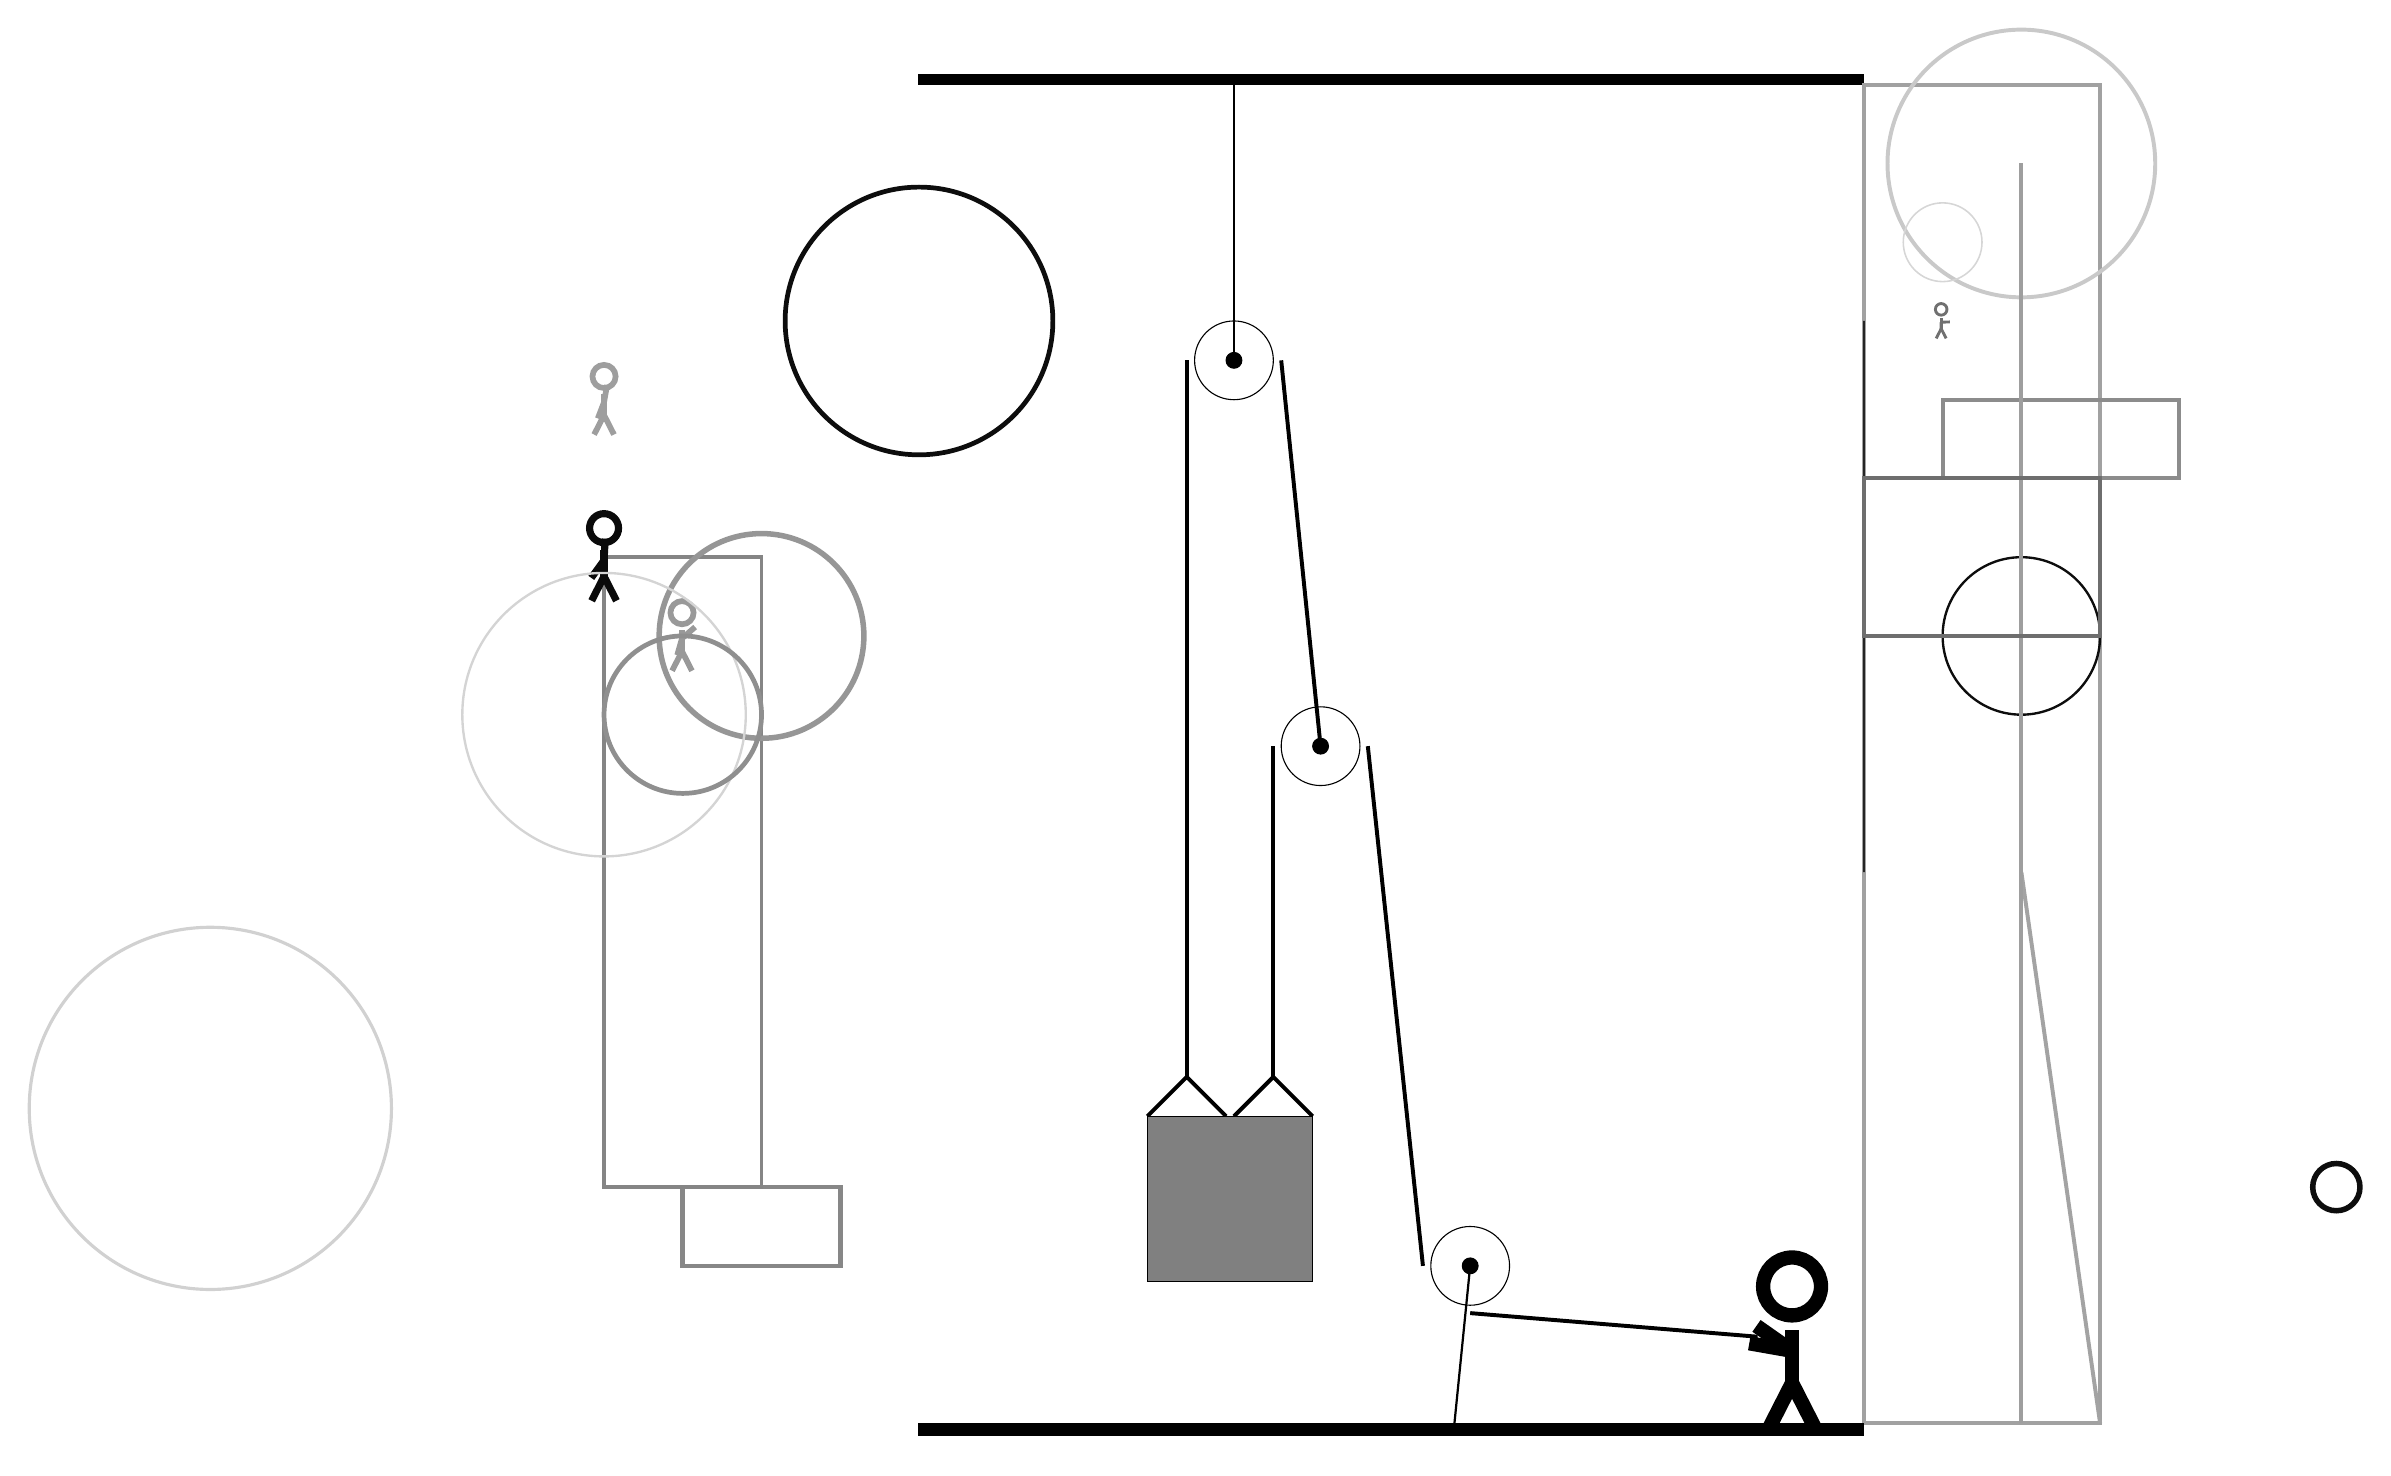
\begin{tikzpicture}
			%%%%% START %%%%%
			
			\draw[fill=black] (-2, 14) rectangle (10, 14.125);
			
			\draw (2, 10.5) circle (0.5);
			\draw[fill=black] (2, 10.5) circle (0.1);
			\draw[thick] (2, 10.5) -- (2, 14);
			
			\draw[line width=0.6mm, color=black!47] (-3, 0) rectangle (-5, -1);
			
			\draw[line width=0.5mm, color=black!37] (10, 14) rectangle (13, -3);
			\node[line width=0.2mm, color=black!40] at (-5, 7) {\Strichmaxerl[4][74][41]};
			\draw [line width=0.6mm, color=black!95](-2, 11) circle (1.7);
			\draw[line width=0.5mm, color=black!36](13, -3) -- (12, 4);
			\draw [line width=0.5mm, color=black!21](12, 13) circle (1.7);
			
			\draw[line width=0.5mm, color=black!48] (-4, 8) rectangle (-6, 0);
			
			\node[line width=0.5mm, color=black!56] at (11, 11) {\Strichmaxerl[2][88][2]};
			\draw[line width=0.3mm, color=black!86] (10, 11) rectangle (10, 4);
			\draw [line width=0.3mm, color=black!95](12, 7) circle (1.0);
			\node[line width=0.7mm, color=black!96] at (-6, 8) {\Strichmaxerl[5][54][87]};
			\draw [line width=0.7mm, color=black!41](-4, 7) circle (1.3);
			\draw[line width=0.5mm, color=black!45] (11, 9) rectangle (14, 10);
			\draw[line width=0.5mm, color=black!38](12, -3) -- (12, 13);
			\draw [line width=0.3mm, color=black!17](-6, 6) circle (1.8);
			\node[line width=0.3mm, color=black!38] at (-6, 10) {\Strichmaxerl[4][69][80]};
			
			\draw [line width=0.4mm, color=black!18](-11, 1) circle (2.3);
			\draw[line width=0.5mm, color=black!57] (10, 7) rectangle (13, 9);
			\draw [line width=0.6mm, color=black!44](-5, 6) circle (1.0);
			
			\draw [line width=0.7mm, color=black!95](16, 0) circle (0.3);
			\draw [line width=0.2mm, color=black!16](11, 12) circle (0.5);
			
			\draw [line width=0.6mm, color=black!13](15, 12) circle (0.0);
			
			\draw (3.1, 5.6) circle (0.5);
			\draw[fill=black] (3.1, 5.6) circle (0.1);
			
			\draw (5, -1) circle (0.5);
			\draw[fill=black] (5, -1) circle (0.1);
			\draw[thick] (5, -1) -- (4.8, -3);
			
			\draw[line width = 0.5mm]  (0.9, 0.9) -- (1.4, 1.4) -- (1.9, 0.9);
			\draw[line width = 0.5mm]  (2.0, 0.9) -- (2.5, 1.4) -- (3.0, 0.9);
			\draw[fill=black!50] (0.9, 0.9) rectangle (3.0, -1.2);
			
			\draw[line width = 0.5mm] (1.4, 10.5) -- (1.4, 1.4);
			\centerarc[line width = 0.5mm](2, 10.5)(0:180:0.6);
			\draw[line width = 0.5mm] (2.6, 10.5) -- (3.1, 5.6);
			\draw[line width = 0.5mm] (2.5, 5.6) -- (2.5, 1.4);
			\centerarc[line width = 0.5mm](3.1, 5.6)(0:180:0.6);
			\draw[line width = 0.5mm] (3.7, 5.6) -- (4.4, -1);
			\centerarc[line width = 0.5mm](5, -1)(180:270:0.6);
			\draw[line width = 0.5mm] (5, -1.6) -- (8.65, -1.9);
			
			\node at (9, -2) {\Strichmaxerl[10][-35][170]};
			
			\draw[fill=black] (-2, -3) rectangle (10, -3.15);
			
			%%%%% END %%%%%
		\end{tikzpicture}
	\end{figure}	
\end{document}